\documentclass[
	10pt,								% globale Schriftgröße
	parskip=half-,						% setzt Absatzabstand hoch
	paper=a4,							% Format
	english,ngerman,					% lädt Sprachpakete
	]{scrartcl}							% Dokumentenklasse

% //////////////////// Pakete laden ////////////////////
\usepackage{amsmath}			% MUSS vor fontspec geladen werden
\usepackage{mathtools}			% modifiziert amsmath
\usepackage{amssymb}			% mathematische symbole, für \ceckmarks
\usepackage{amsthm}				% für proof
\usepackage{mathrsfs}			% für \mathscr
\usepackage{latexsym}
\usepackage{marvosym}				% für Lightning

\usepackage{fontspec} 			% funktioniert nur mit den neueren Compilern z.B. XeLaTeX
\usepackage{microtype}			% für bessere Worttrennung
\usepackage[ngerman]{babel} 	% Spracheinstellung
\usepackage{lmodern}			% verändert verwendete Schriftart, damit sie weniger pixelig ist

\usepackage{verbatim}
\usepackage{listings}			% Für Quellcode

\usepackage{graphicx}
\usepackage{tabularx}			% für Tabellen mit gleicher Spaltenbreite und automatischen Umbrüchen
\usepackage{fullpage}
\usepackage{multirow}			% für multirow in tabulars
\usepackage{rotate}
\usepackage[cmyk,table]{xcolor} % um Farben zu benutzen, kann mehr als das Paket color
\usepackage[					% Verlinkungen
	colorlinks,					% farbige Schrift, statt farbiger Rahmen
	linktocpage,				% verlinkt im Abb.Verzeichnis Seitenzahl statt Bildunterschrift
	linkcolor=blue				% setzt Farbe der Links auf blau
	]{hyperref}					% nur für digitale Anwendungen, url = "http://www.example.com"
\usepackage{url}				% für Webadressen wie e-mail usw.: "\url{http://www.example.com}"

\usepackage{enumerate}			% für versch. Aufzählungezeichen wie z.B. a)
\usepackage{xspace}				% folgt ein Leerzeichen nach einem \Befehl, wird es nicht verschluckt.
\usepackage{cancel}				% für das Durchstreichen u.a. in Matheformeln mit \cancel
\usepackage{float}              % zum Forcieren der Position von figure-Umgebungen

% zum Zeichnen (u.a. von Graphen)
\usepackage{fp}
\usepackage{tikz}
\usetikzlibrary{tikzmark}			% für \tikzmark{toRemember}
\usetikzlibrary{positioning}	% verbesserte Positionierung der Knoten
\usetikzlibrary{automata}		% für Automaten (GTI)
\usetikzlibrary{arrows}
\usetikzlibrary{shapes}
\usetikzlibrary{decorations.pathmorphing}
\usetikzlibrary{decorations.pathreplacing}
\usetikzlibrary{decorations.shapes}
\usetikzlibrary{decorations.text}

% //////////////////// Syntaxhighlighting ////////////////////
\lstloadlanguages{Python, Haskell, [LaTeX]TeX, Java}
\lstset{
   basicstyle=\footnotesize\ttfamily,	% \scriptsize the size of the fonts that are used for the code
   backgroundcolor = \color{bgcolour},	% legt Farbe der Box fest
   breakatwhitespace=false,	% sets if automatic breaks should only happen at whitespace
   breaklines=true,			% sets automatic line breaking
   captionpos=t,				% sets the caption-position to bottom, t for top
   commentstyle=\color{codeblue}\ttfamily,% comment style
   frame=single,				% adds a frame around the code
   keepspaces=true,			% keeps spaces in text, useful for keeping indentation
							% of code (possibly needs columns=flexible)
   keywordstyle=\bfseries\ttfamily\color{codepurple},% keyword style
   numbers=left,				% where to put the line-numbers;
   							% possible values are (none, left, right)
   numberstyle=\tiny\color{codegreen},	% the style that is used for the line-numbers
   numbersep=5pt,			% how far the line-numbers are from the code
   stepnumber=1,				% nummeriert nur jede i-te Zeile
   showspaces=false,			% show spaces everywhere adding particular underscores;
							% it overrides 'showstringspaces'
   showstringspaces=false,	% underline spaces within strings only
   showtabs=false,			% show tabs within strings adding particular underscores
   flexiblecolumns=false,
   tabsize=1,				% the step between two line-numbers. If 1: each line will be numbered
   stringstyle=\color{orange}\ttfamily,	% string literal style
   numberblanklines=false,				% leere Zeilen werden nicht mitnummeriert
   xleftmargin=1.2em,					% Abstand zum linken Layoutrand
   xrightmargin=0.4em,					% Abstand zum rechten Layoutrand
   aboveskip=2ex, 
}

\lstdefinestyle{py}{
   language=Python,
}
\lstdefinestyle{hs}{
   language=Haskell,
}
\lstdefinestyle{tex}{
	language=[LaTeX]TeX,
	escapeinside={\%*}{*)},     % if you want to add LaTeX within your code
	texcsstyle=*\bfseries\color{blue},% hervorhebung der tex-Schlüsselwörter
	morekeywords={*,$,\{,\},\[,\],lstinputlisting,includegraphics,
	rowcolor,columncolor,listoffigures,lstlistoflistings,
	subsection,subsubsection,textcolor,tableofcontents,colorbox,
	fcolorbox,definecolor,cellcolor,url,linktocpage,subtitle,
	subject,maketitle,usetikzlibrary,node,path,addbibresource,
	printbibliography},% if you want to add more keywords to the set
     numbers=none,
     numbersep=0pt,
     xleftmargin=0.4em,
}

\lstdefinestyle{java}{
	language=Java,
	extendedchars=true,		% lets you use non-ASCII characters;
   						% for 8-bits encodings only, does not work with UTF-8
}

\lstdefinelanguage[x64]{Assembler}     % add a "x64" dialect of Assembler
   [x86masm]{Assembler} % based on the "x86masm" dialect
   % with these extra keywords:
   {morekeywords={CDQE,CQO,CMPSQ,CMPXCHG16B,JRCXZ,LODSQ,MOVSXD, %
                  POPFQ,PUSHFQ,SCASQ,STOSQ,IRETQ,RDTSCP,SWAPGS, %
                  rax,rdx,rcx,rbx,rsi,rdi,rsp,rbp, %
                  r8,r8d,r8w,r8b,r9,r9d,r9w,r9b}
}					% for 8-bits encodings only, does not work with UTF-8

\lstdefinestyle{c}{
	language=c,
	extendedchars=true,		% for 8-bits encodings only, does not work with UTF-8
}

% //////////////////// eigene Kommandos ////////////////////
\newcommand\FU{Freie Universität Berlin\xspace}% benötigt package xspace
\newcommand\gdw{g.\,d.\,w.\xspace}
\newcommand\oBdA{o.\,B.\,d.\,A.\xspace}
\newcommand{\Eu}{\texteuro}
\newcommand\N{\mathbb{N}\xspace}
\newcommand\Q{\mathbb{Q}\xspace}
\newcommand\R{\mathbb{R}\xspace}
\newcommand\Z{\mathbb{Z}\xspace}
\newcommand\ohneNull{\ensuremath{\backslash\lbrace 0\rbrace}}% \{0}
\let\dhALT\dh	% Schreibt Befehl \dh in \dhALT um
\renewcommand\dh{d.\,h.\xspace}	%renew überschreibt command \dh
\newcommand\Bolt{\;\text{\LARGE\raisebox{-0.3em}{\Lightning}\normalsize}\xspace}% Blitz
\newcommand\zz{\ensuremath{\raisebox{+0.25ex}{Z}% zu zeigen
			\kern-0.4em\raisebox{-0.25ex}{Z}%
			\;\xspace}}
\newcommand{\from}{\ensuremath{\colon}}
\newcommand{\floor}[1]{\lfloor{#1}\rfloor}
\newcommand{\ceil}[1]{\lceil{#1}\rceil}
 \renewcommand{\L}{\ensuremath{\mathcal{L}}\xspace}
 \renewcommand{\P}{\ensuremath{\mathcal{P}}\xspace}
 \newcommand{\NL}{\ensuremath{\mathcal{N}\kern-0.2em\mathcal{L}}\xspace}
 \newcommand{\NP}{\ensuremath{\mathcal{NP}}\xspace}

% //////////////////// Mathefunktionen ////////////////////
\DeclareMathOperator{\Landau}{\mathcal{O}}
\DeclareMathOperator{\True}{True}
\DeclareMathOperator{\False}{False}

% //////////////////// eigene Theoreme ////////////////////
\newtheorem{theorem}{Satz}
\newtheorem{corollary}[theorem]{Folgerung}
\newtheorem{lemma}[theorem]{Lemma}
\newtheorem{observation}[theorem]{Beobachtung}
\newtheorem{definition}[theorem]{Definition}
\newtheorem{Literatur}[theorem]{Literatur}
% konfiguriert proof
\makeatletter
\newenvironment{Proof}[1][\proofname]{\par
  \pushQED{\qed}%
  \normalfont \topsep6\p@\@plus6\p@\relax
  \trivlist
  \item[\hskip\labelsep
%         \itshape
        \bfseries
    #1\@addpunct{.}]\ignorespaces
}{%
  \popQED\endtrivlist\@endpefalse
}
\makeatother

% //////////////////// eigene Farben ////////////////////
\let\definecolor=\xdefinecolor
\definecolor{FUgreen}{RGB}{153,204,0}
\definecolor{FUblue}{RGB}{0,51,102}

\definecolor{middlegray}{rgb}{0.5,0.5,0.5}
\definecolor{lightgray}{rgb}{0.8,0.8,0.8}
\definecolor{orange}{rgb}{0.8,0.3,0.3}
\definecolor{azur}{rgb}{0,0.7,1}
\definecolor{yac}{rgb}{0.6,0.6,0.1}
\definecolor{Pink}{rgb}{1,0,0.6}

\definecolor{bgcolour}{rgb}{0.97,0.97,0.97}
\definecolor{codegreen}{rgb}{0,0.6,0}
\definecolor{codegray}{rgb}{0.35,0.35,0.35}
\definecolor{codepurple}{rgb}{0.58,0,0.82}
\definecolor{codeblue}{rgb}{0.4,0.5,1}

% //////////////////// eigene Settings ////////////////////

\textheight = 230mm		% Höhe des Satzspiegels / Layouts
\footskip = 10ex			% Abstand zw. Fußzeile und Grundlinie letzter Textzeile
\parindent 0pt			% verhindert Einrückung der 1. Zeile eines Absatzes
\setkomafont{sectioning}{\rmfamily\bfseries}% setzt Ü-Schriften in Serifen, {disposition}											% bindet Header ein (WICHTIG)
\usepackage{graphicx}

\newcommand{\dozent}{Prof.  Dr.  Agnès Voisard, Nicolas Lehmann}					% <-- Names des Dozenten eintragen
\newcommand{\tutor}{Hoffman Christian}						% <-- Name eurer Tutoriun eintragen
\newcommand{\tutoriumNo}{Tutorium 3}				% <-- Nummer im KVV nachschauen
\newcommand{\projectNo}{1}									% <-- Nummer des Übungszettels
\newcommand{\veranstaltung}{Datenbank Systeme}	% <-- Name der Lehrveranstaltung eintragen
\newcommand{\semester}{SoeSe 2017}						% <-- z.B. SoSo 17, WiSe 17/18
\newcommand{\studenten}{Ingrid Tchilibou, Emil Milanov, Boyan Hristov}			% <-- Hier eure Namen eintragen
% /////////////////////// BEGIN DOKUMENT /////////////////////////


\begin{document}
% /////////////////////// BEGIN TITLEPAGE /////////////////////////
\begin{titlepage}
	\subject{\dozent}
	\title{\veranstaltung, \semester}
	\subtitle{\Large Project \projectNo\\ \large\vspace{1ex} TutorIn: \tutor\\ Tutorium \tutoriumNo}
	\author{\studenten}
	\date{\normalsize \today}
\end{titlepage}

\maketitle								% Erstellt das Titelblatt
\vspace*{-10cm}							% rückt Logo an den oberen Seitenrand
\makebox[\dimexpr\textwidth+1cm][r]{	%rechtsbündig und geht rechts 1cm über Layout hinaus
	
\includegraphics[width=0.4\textwidth]{src/fu_logo} % fügt FU-Logo ein
}
% /////////////////////// END TITLEPAGE /////////////////////////

\vspace{7cm}							% Abstand
\rule{\linewidth}{0.8pt}				% horizontale Linie										% erstellt die Titelseite


% /////////////////////// Aufgabe 1 /////////////////////////
\section{Aufgabe: Projektdokumentation}
Link zum Projekt: \url{https://github.com/gancia-kiss/dbs_projekt}

Das Team: Emil Milanov, Boyan Hristov, Ingrid Tchilibou\\
Wir sind alle Bachelor Informatik Studenten im 4. Semester.

\textbf{Projektziel}\\
Unserer Meinung nach hat dieses Projekt als Ziel Verhältnisse zwischen Tweets und Hashtags oder zwischen Paaren von Hashtag zu 
analysieren und auch grafisch darzustellen. Laut der Aufgabenstellung soll das eine Web-Anwendung sein, was wir uns merken 
müssen, ist aber in der ersten Projektiteration nicht wichtig. 


\textbf{Aufgabenverteilung}\\
Alle drei von uns haben gründlich das ER Modell besprochen und mit Aufmerksamkeit eine Eintscheidung getroffen. Ingrid hat zusätzlich die Daten gründlich analysiert, Emil und Ingrid haben das relationales Modell erstellt und Boyan hat das ER Modell gezeichnet und bereinigt, die Datenbank mithilfe von Postgres erstellt und eine Möglichkeit gefunden, eine Dumpdetei zu erstellen, als Beweis, dass wir eine Datenbank fertig haben. Zusätzlich haben Emil und Ingrid die Dokumentationn verfasst.



% ///////////////////// Aufgabe 2 ///////////////////
\section{Aufgabe:Explorative Datenanalyse}

Wir haben eine Tabelle mit 10 Attributen von verschiedenen Tweets von der 2016 America Election.\\
Jeder Tupel beschreibt genau :\\

Von wem wurde den Tweet gepostet? Dafür gibt es den Attribut {\itshape Handle}\\
Was war die Nachricht / Inhalt von diesem Tweet? Dafür ist den Attribut {\itshape Text}\\
Manche posts von Trump und Clinton waren eigentlich Retweets von Tweets von anderen Personen.
Dafür wird den Attribut Original Author erstelt.
Außerdem hat jeder Tweet einen {\itshape Source-url} als Attribut (D.h Was für ein Platform oder Gerät benutzt wurde, um den Tweet zu veröffentlichen)\\
Wie häufig wurde diesen Tweet weitergeleitet?  {\itshape retweet-count}\\
Wie häufig wurde diesen Tweet \"geliked\" oder gespeichert. {\itshape favorite-count }?\\

Außerdem gibt es Tweets, die ein Zitat enthalten. Dieses Zität wird als Anhang im Browser angezeigt, aber wird nicht vom API genommen. Solche Tweets sind auch truncated oder abgeschnitten. {\itshape is-quote status}\\
Zusätzlich gibt es auch manche Tweets, die 'truncated' worden sind. Das heißt, dass die ein zitiertes Tweet oder irgendwelche Media enthalten, deswegen überschritten sie das Twitter Zeichenlimit und werden abgeschnitten.\\ 

Für uns wären {\itshape text}, {\itshape handle}, {\itshape time}, {\itshape retweet-count} und {\itshape favourite-count} besonders wichtig, da man mit diesen Daten alle von den gegebenen möglichen Anfragen bearbeiten kann. Das Attribut {\itshape text} enthält alle HashTags und es gibt leider kein anderes Attribut dazu, deswegen werden wir die HashTags von diesem Attribut nehmen. Wie schon erwähnt, müssen wir hier auf das Attribut {\itshape truncated} aufpassen. \\

Für die Wichtigkeit des Tweets könnte im unseren Fall auch wichtig sein, ob Trump oder Clinton Tweets weitergeleitet haben. Dafür ist das Attribut {\itshape  original author}. Öftmals sind das Tweets mit 'trending' Messages/Aussagen. 

\section{Aufgabe: ER-Modelierung}

Alle drei von uns haben dieses Modell gründlich besprochen und eine Entscheidung getroffen. Wir glauben, dass dieses Modell das beste für unsere Vorstellung des Projekts ist.

\textbf{Probleme und Lösungen}\\

\begin{itemize}
 \item Um 'Welche Hashtags werden am meistens verwendet' zu beantworten, muss man für jeden Hashtag überprüfen, in welchen Tweets er vorkommt und dann diese aufzählen. Deswegen haben wir uns entschieden, in dem Hashtah Entitätstyp ein Attribut TotalCount zu speichern. So werden wir auch weniger Server-Anfragen bearbeiten müssen.
 
 \item Der Datenumfang ist über mehreren Monaten. Um die Fragen 'Wann traten insgesammt am meisten Hashtags auf?' und 'Wie hat sich die Häufigkeit der Verwendung eines speziellen Hashtags im Laufe der Zeit entwickelt?' zu beantworten müssen wir jeden Tweet zu einem zeitlichen Bereich zuordnen. 
 
 Wir haben uns deswegen entschieden, einen Entitätstyp 'Week' zu haben, wo wir an einer Woche benutzten Hashtags speichern werden. (Natürlich auch einen Attribut "Count" für höhere effizienz verwenden)
 
 \item Unserer Meinung nach, wäre eine Metrik für wichtige Tweets die Summe von Retweets und Favourites. So haben wir einen Attribut 'Rating', der nach der folgende Schema berechnet wird;
 
 \begin{center}
 $retweets*weight_1 + favourites*weight_2 = rating$ 
 \end{center}
 
 wobei $weight_1$ und $weight_2$ später genau bestimmt werden.

 \item Es wird ziemlich aufwändig herauszufinden, welche Paar von Hashtags am häufigsten gemeinsam auftritt, weil wir über alle Tweets iterieren müssen. Deswegen haben wir eine N:M rekursive Relation auf 'Hashtag' erstellt.
 
 \item Eigentlich haben wir zu fast jedem Entitätstyp einen Attribut 'count' hinzugefügt, weil die Berechnung von Anzahl viel einfacher zu Parse-Zeit wäre, als jedes mal eine Anfrage zu machen, und dann alle verschiedene Entitäten aufzuzählen.
 
\end{itemize}

\vspace{1cm}
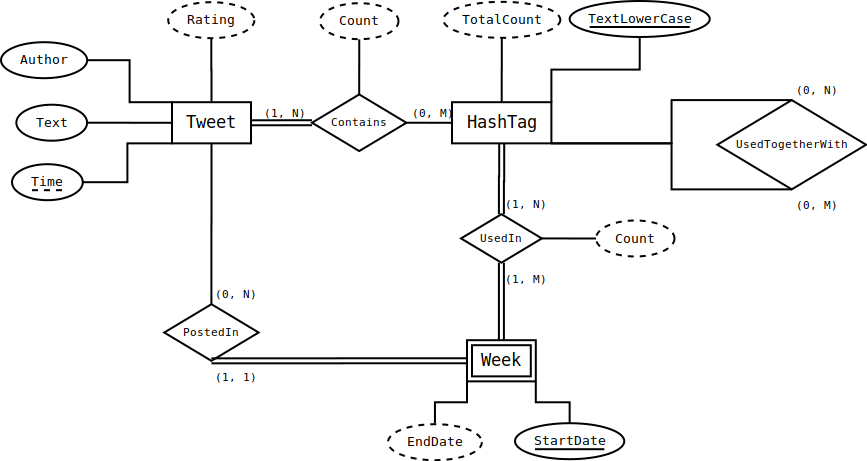
\includegraphics[width=\textwidth]{ERDiagramm.png}

\section{Aufgabe: Relationales Modell}

Nachdem wir die ER Diagramm hatten, war es einfach ein relationelles Modell zu erstellen. Aufgrund der Aufgabestellung 
und unsere Interpretation, sind nicht alle Attribute aus der .csv Datei für uns Relevant. Im 3. Teil der Projektdokumentation
sind unsere Probleme, Lösungen und Entscheidungen um den Entitätstypen und deren Attributen zu sehen. Trotzdem war es 
für uns sehr einfach ein relationelles Modell zu erstellen.

Einige Entscheidungen, die wir bei der Erstellung des relationalen Modell treffen müssten waren z.B in welcher Tabelle die 
verschiedene 'Count' Attributen sein müssen.

Unsere Haupttabellen sind TWEET, HASHTAG und WEEK, jede von denen einen ID Attribut hat, und HASHTAG.Text wird nur kleine 
Buchstaben haben. 

Wir vermuten auch zum Beispiel, dass Hashtags maximal 40 Zeichen lang sind. Natürlich gibt es längere Hashtags, aber wir glauben 
dass Trump und Clinton keine solche Hashtags verwenden. Für Handle brauchen wir nicht mehr als 20 Zeichen. Normalerweise sind 
Tweets maximal 200 Zeichen lang, es gibt aber manche, die Truncated worden sind und es zusätzlich eine Link enthalten, was 
die Grenze überschritten kann. Deswegen haben wir uns entschieden 200 Zeichen für jeden Tweet zu speichern.

Tweet(\underline{ID :: integer}, Handle :: character varying(20), Text :: character varying(200), \\
	\hspace*{10mm} Time :: date, Rating :: integer, Count :: integer, replyTo :: character varying(20), \\
    \hspace*{10mm} isRetweet :: boolean, isQuote :: boolean, isTruncated :: boolean ) \\
    
Hashtag(\underline{TextLowerCase :: char varying(40)}, TotalCount :: integer) \\
Week(\underline{StartDate :: date}, EndDate :: date) \\

Contains(\underline{Tweet.ID, Hashtag.TextLowerCase}) \\
UsedIn(\underline{Week.StartDate, Hashtag.ID}, Count :: integer) \\
WeeklyTweers(\underline{Week.StartDate , Hashtag.ID}) \\ 
UsedTogetherWith(\underline{HT1.ID, HT2.ID}) \\



\section{Aufgabe: Datenbank erstellen}
Wir sind nicht sicher wie wir beweisen können, dass wir die Datenbank erstellt haben, deswegen wenn man den Link öffnet, 
sind ein paar Screenshots zu finden. Außerdem steht im Github-repo eine .sql Datei, wo mann alle bei der Erstellung der Datenbank
ausgeführte Anweisungen finden kann. 

Trotzdem, nachdem wir ein relationales Modell hatten, war es einfach die Datenbank zu erstellen. Das schwierigste bei diesem Teil
der Aufgabe war zu lernen, wie man mit Postgres umgeht.

Wir haben alle Tabellen, als auch die Relationen dazwischen erstellt. Falls das aber nicht notwendig ist, hier sind die notwendige Befehle, die wir ausgeführt haben, um unsere Datenbank zu erstellen aus dem Arch Linux wiki:

sudo -u postgres -i
initdb --locale \$LANG -E UTF8 -D '/var/lib/postgres/data' \\

Das wechselt zu dem default postgre Nutzer und erstellt den Datenbank cluster \\

createuser --interactive hristov \\

Das erstellt ein postgresql Nutzer. Hier ist es klever das selbe Nutzername als das eigene auf dem Rechner zu nutzen um Authentifizierung zu erleichtern. \\

createdb Election \\

Das erstellt ein Datenbank mit dem Namen 'Election' \\

psql -d Election \\

So geht man in dem Shell von dem Datenbank rein. Danach kann man SQL Befehle benutzen um 
Tabellen zu erstellen, Daten aufzurufen und im großen und ganzen alles was man sonst mit SQL machen darf. Am Ende kann man auch die für die Erstellung benutze Befehle exportieren und das ganze Datenbank migrieren. Das haben wir auch als Beweis gemacht.

pg\_dump Election > Election.sql


% /////////////////////// END DOKUMENT /////////////////////////
\end{document}